\documentclass[11pt]{article}
%\documentclass[draft]{article} for better debugging!

\usepackage{cite}
\usepackage{graphicx}
%download float barrier sty - uni mail
\linespread{1.3}

\addtolength{\textwidth}{2cm}
\addtolength{\hoffset}{-1cm}


\addtolength{\textheight}{2cm}
\addtolength{\voffset}{-1cm}

\begin{document}


\subsection{Bacteria colonise lipids in activated sludge}
It was essential to establish an experimental parameters and adapt protocols to observe the impact of lipids on activated sludge before a controlled enrichment experiment could be conducted. Hence a trial run preceded the actual enrichment run. The trial was conducted with 1 \% GT  addition to sludge replicates and sampling frequency was every 7 days as the expectation was that the enrichment would run for an extended period of time. GT formed a transparent and hydrophobic layer on the surface of the enrichment cultures, which was replaced with white droplets suspended below the culture surface within 7 days. Whilst varied in size the droplet consistently decreased in diameter with increased incubation period until the they were indistinguishable from the sludge after 21 days. Droplet formation decreased floc settlement for the duration of their presence. 

\subsubsection{\emph{change in morphology}}
\begin{figure}
\includegraphics[scale=.9]{cultures.jpg}
\caption{Impact of lipid addition to activated sludge cultures}
\end{figure}


\subsubsection{\emph{Microscopy}}
 Droplets were isolated and stained with SybrGreen before imaging with epifluorescence microscopy (\textbf{Figure 1}). 

\begin{figure}
\includegraphics[scale=.4]{august_microscopy.png}
\caption{Imaging of washed lipid droplets post SybrGreen staining via fluorescence microscopy. The dye stains DNA green, lipid appears yellow. \textit{A}) shows inorganic matter which appears orange; \textit{B}), \textit{C}) and \textit{D}) show bacterial attachment to lipid substrates \textit{E}) \textit{F}).}
\end{figure}


\textbf{Figure xx } shows biomass attached to lipid droplets. As the lipid droplets were washed twice before staining and imaging, the biomass is firmly attached to the droplets. \textbf{Figure 1}\textit{B} and \textbf{Figure 1}\textit{D} show cells colonising the surface of a lipid droplet. \textbf{Figure 1}\textit{C} shows cells internal to the lipid droplet.

\subsubsection{\emph{Monitoring lipase production}}
Lipase was activity was detected upon colorimetric change from p-nitrophenyl palmitate cleavage in the substrate solution. The assay separated  EC, EPS bound and cell membrane bound lipases from each enrichment (\textbf{Graph 2}).

\begin{figure}
\includegraphics[scale=1]{lip_av.PNG}
\caption{Total lipase activity of all fractions and replicates}
\end{figure}

\begin{figure}
\includegraphics[scale=1.1]{lip_sn.PNG}
\caption{Average lipase activity in the supernatant fraction}
\end{figure}

\begin{figure}
\includegraphics[scale=1.1]{lip_eps.PNG}
\caption{Average lipase activity in the EPS fraction}
\end{figure}

\begin{figure}
\includegraphics[scale=1.1]{lip_biom.PNG}
\caption{Average lipase activity in the biomass fraction}
\end{figure}

%\begin{figure}
%\includegraphics[scale=1]{lipase_activity.png}
%\caption{Shows the comparative average lipase activity after 8 and 15 days of incubation for the different lipases in each enrichment.}
%\end{figure}


It is evident from  \textbf{Graph 2} that membrane bound lipase is the most abundant across all enrichment cultures at both time points, where highest activity was recorded in no treatment, followed by the acetate enrichment and then GT enrichment.  The activity for the 8 day time point was close to synonymous with the 15 day time point, with highest difference of 0.1 seen in GT membrane lipase activity.

\subsection{Lipid colonising isolates behave differently in the presence of lipids}
% change in morphology in LC1 and LuxR data

\begin{figure}
\includegraphics[scale=1.1]{LCM_LuxR.png}
\caption{Response to LuxR bioassay by lipid colonising isolates, comparatively cultured in the presence and absence of lipid }
\end{figure}


\subsection{Micobial community changes in the presence of lipids}
%DGGE and sequencing data

\begin{figure}
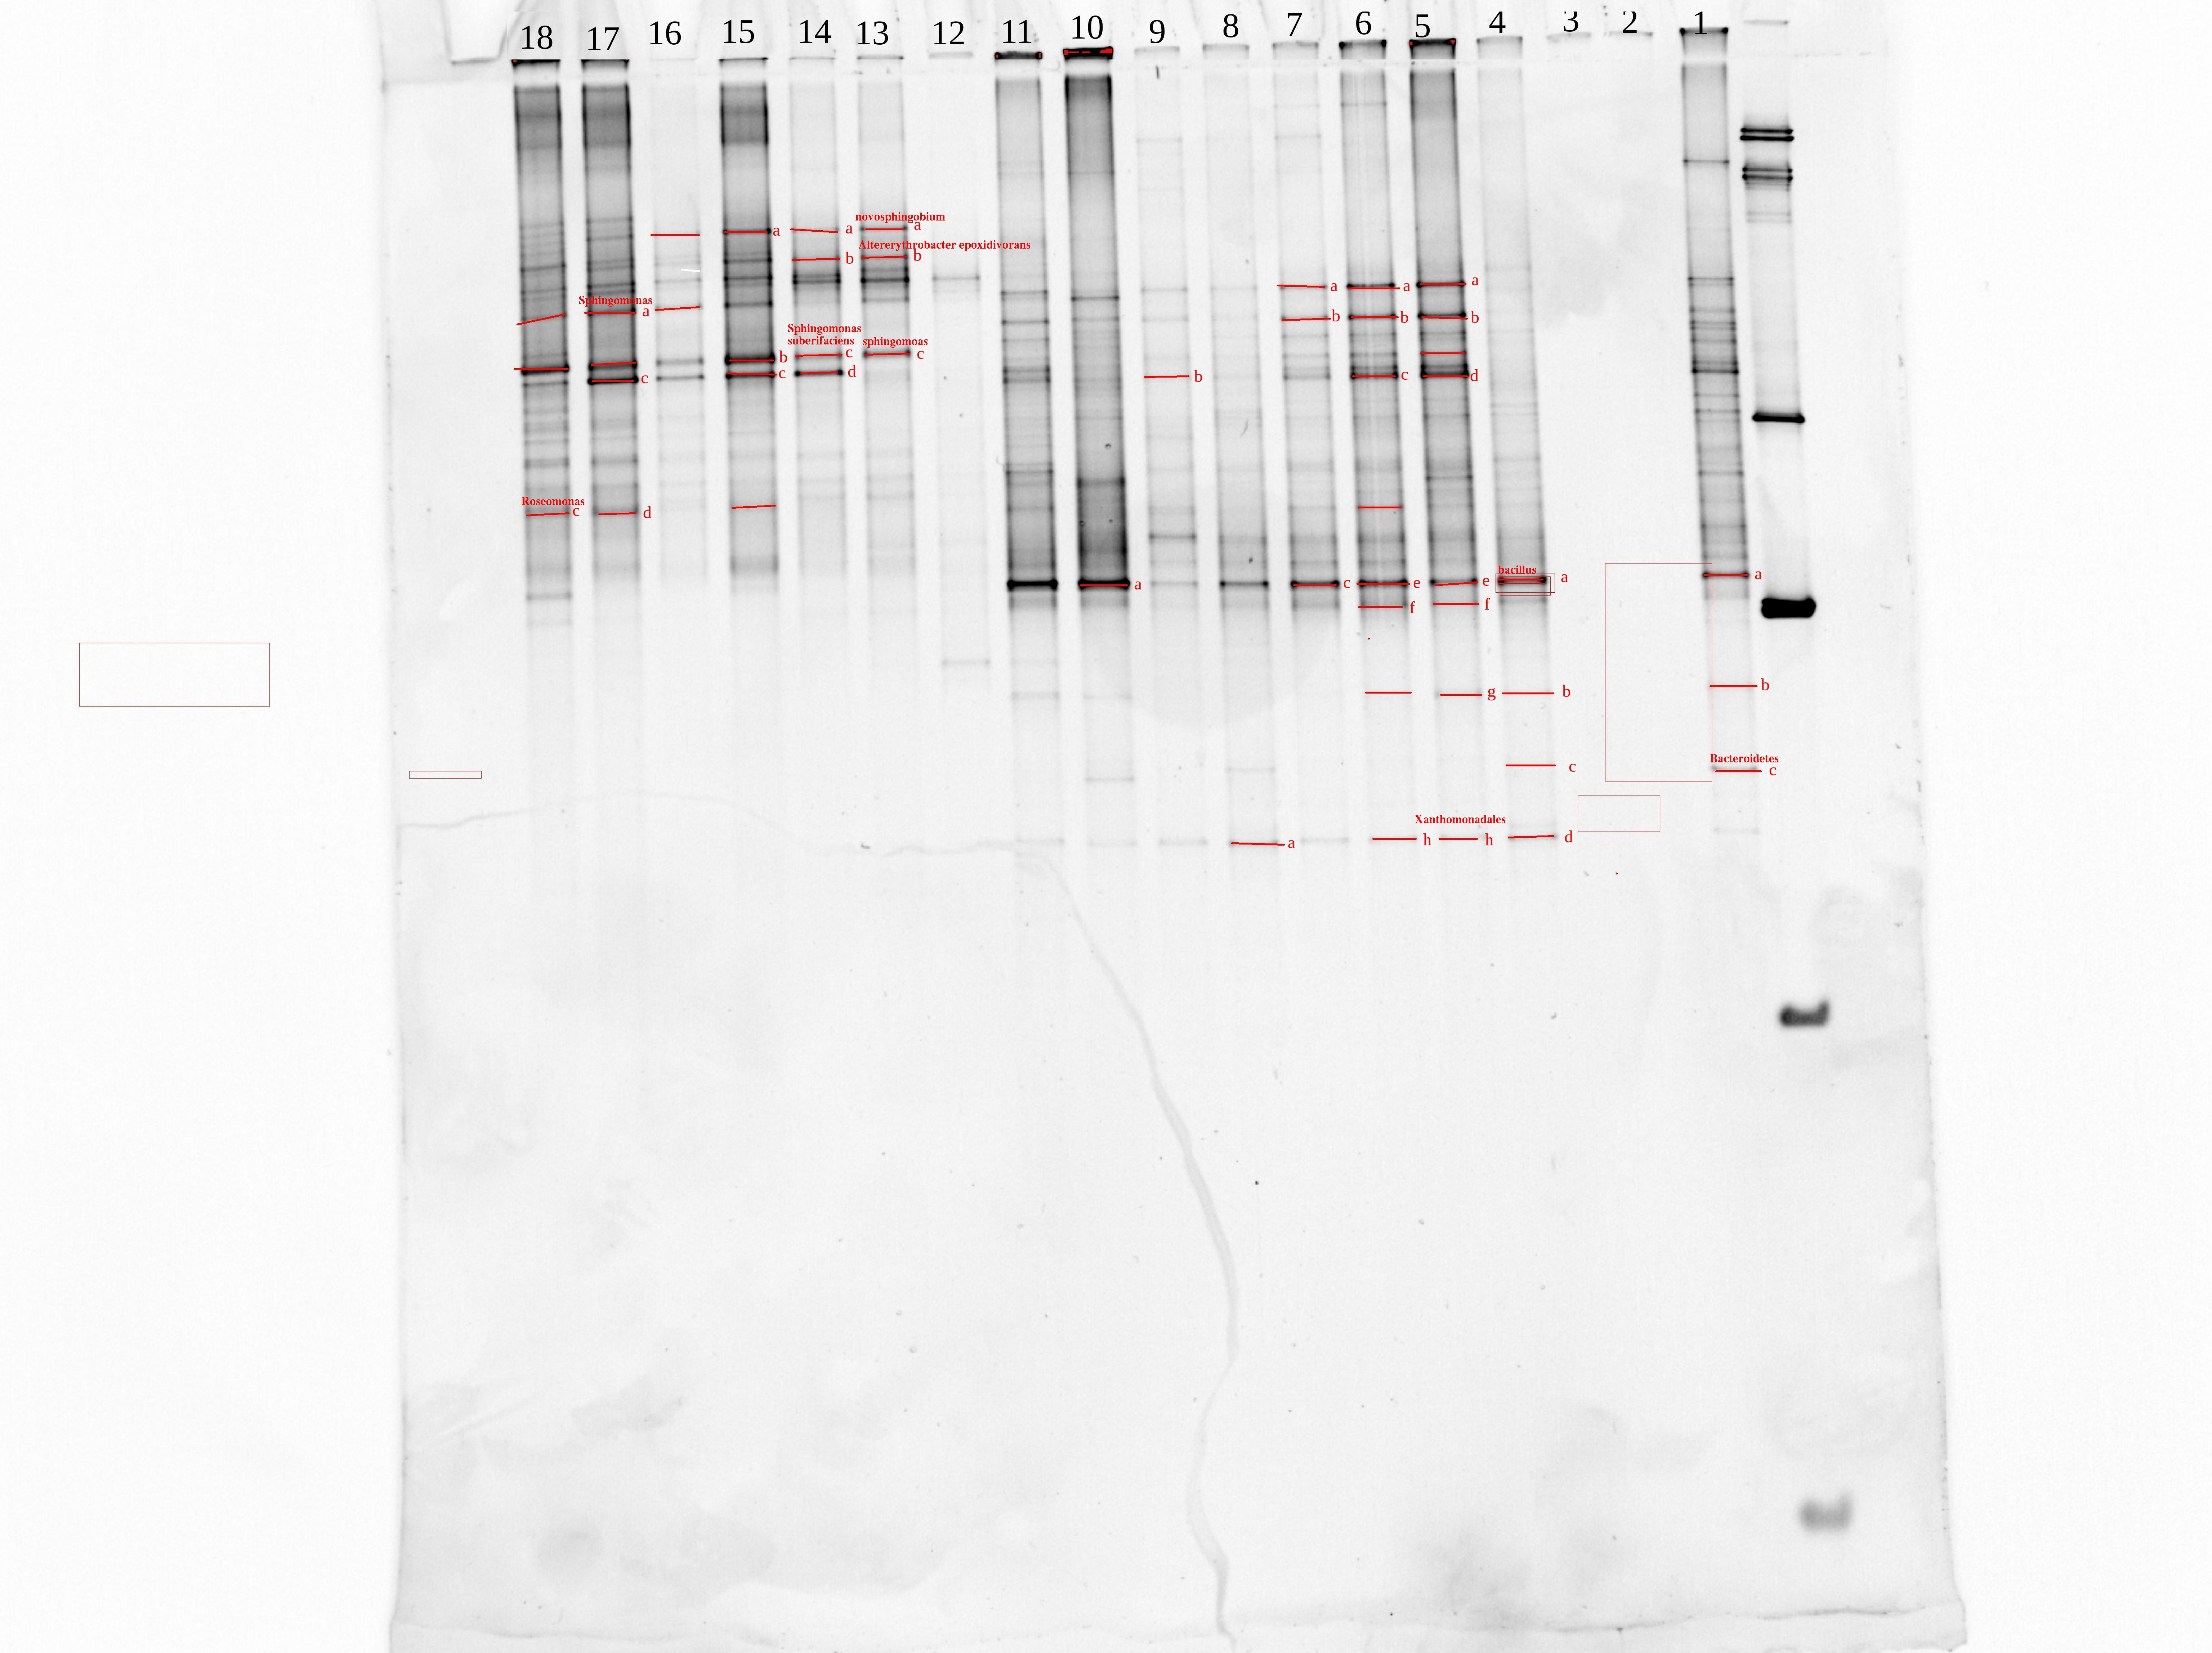
\includegraphics[scale=.5]{DGGE_R4_450bp_annotated_w_BLAST.jpg}
\caption{Community structure of control and enriched cultures of replicate 4}
\end{figure}

\begin{figure}
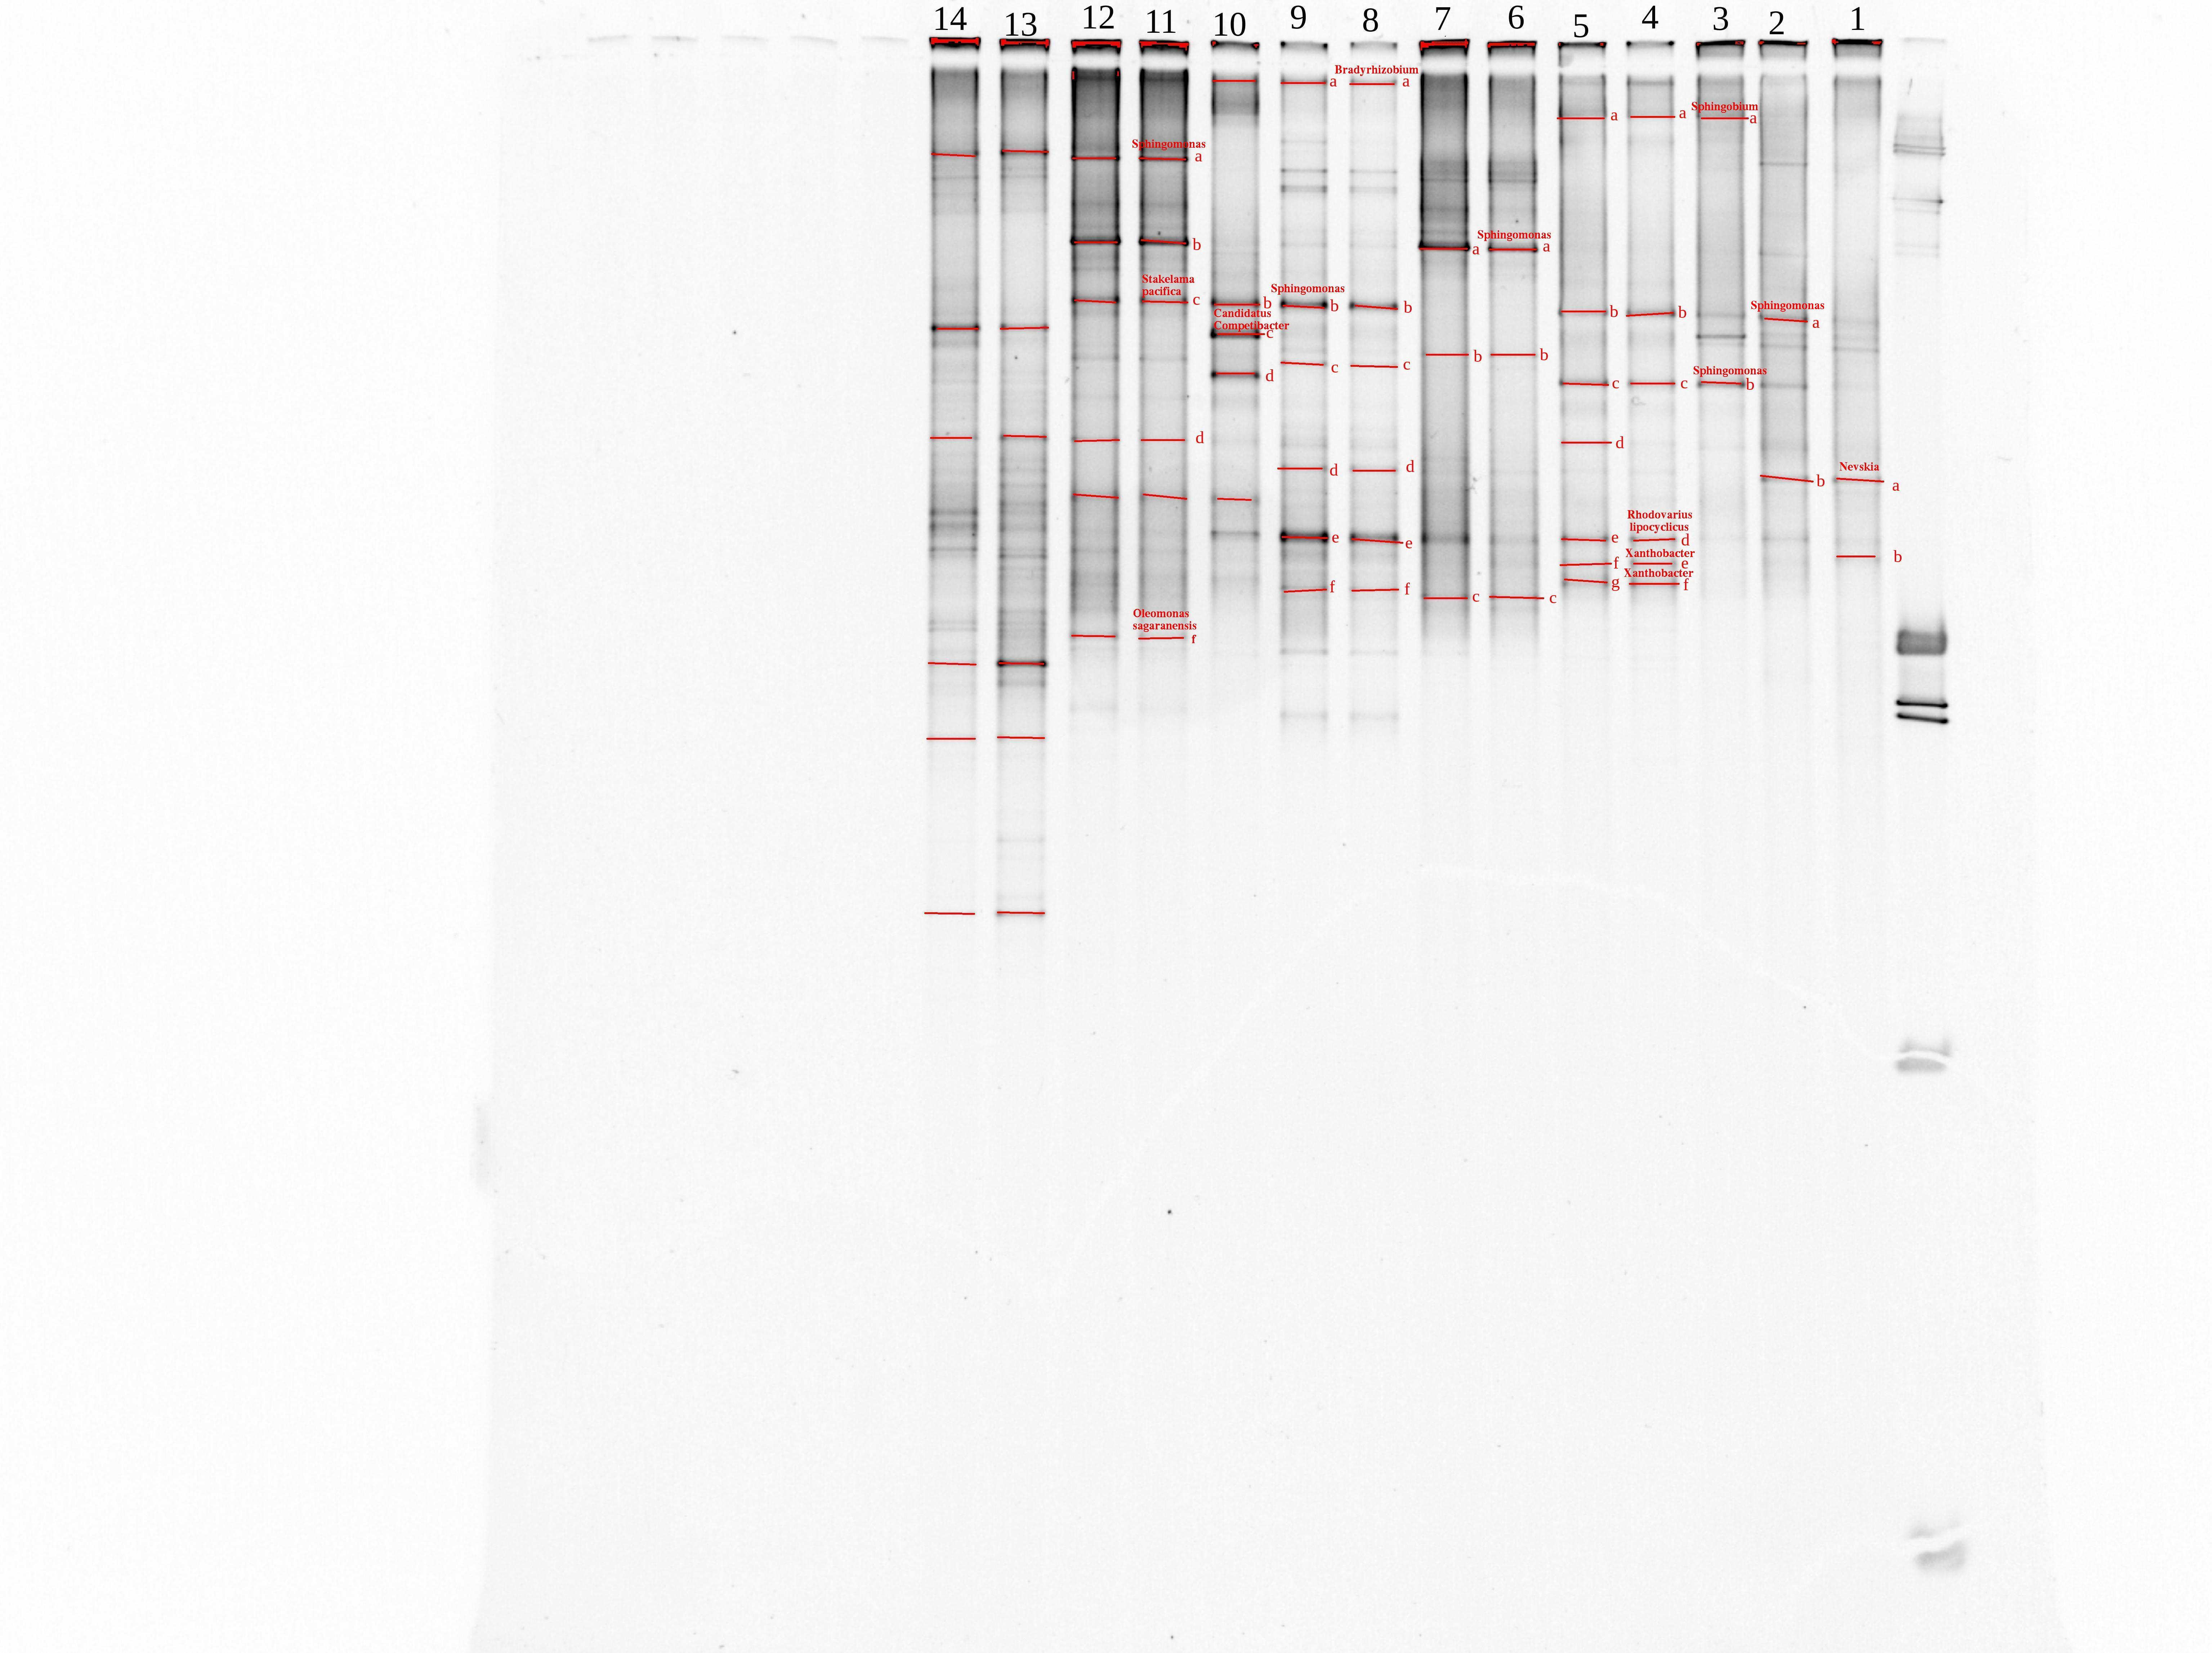
\includegraphics[scale=.5]{DGGE_misc_450bp_annotated_w_BLAST.jpg}
\caption{Community structure of aggregates, emulsions, secondary and tertiary enrichments}
\end{figure}

\end{document}